\chapter{Fundamentação Teórica}\label{cap:fundamentacao}

Neste capítulo, são apresentados os conceitos e as definições necessárias para o entendimento deste trabalho. A Seção \ref{sec:osteoartrite} apresenta a osteoartrite de joelhos e suas características clínicas. A seção \ref{sec:visao-computacional} aborda a visão computacional na área da saúde. A Seção \ref{sec:aprendizado-profundo} mostra alguns conceitos fundamentais de arquiteturas de aprendizado profundo, incluindo as redes neurais convolucionais e os vision transformers.

% Por fim, a seção \ref{sec:ajuste-fino} apresenta os conceitos de transferência de aprendizado através do ajuste fino de modelos pré-treinados.

\section{Osteoartrite de Joelho}\label{sec:osteoartrite}

\subsection{Definição e Características Clínicas}

A osteoartrite (OA) é definida como uma doença heterogênea e degenerativa, que afeta as articulações e estruturas ósseas de pacientes, causando sintomas de dor, deformidade e perda de função \citep{Loeser2012}. Considerando os fenótipos da doença, ou seja, as características clínicas e radiográficas observáveis, a OA é considerada altamente heterogênea, isso significa que pode ser causada por diversos fatores, incluindo:

\begin{itemize}
    \item \textbf{Idade}: a OA é mais comum em idosos, devido ao desgaste natural e inevitável das articulações ao longo do tempo \citep{ShaneAnderson2010}.
    \item \textbf{Sexo}: mulheres têm maior risco de desenvolver OA do que homens, especialmente após a menopausa, devido à diminuição dos níveis de estrogênio, que protege a cartilagem articular \citep{Tschon2021}.
    \item \textbf{Obesidade}: o excesso de peso também é uma condição de risco para a OA, pois aumenta a carga mecânica nas articulações, influenciando o início e a progressão da doença \citep{PACCA2018}.
    \item \textbf{Predisposição genética}: fatores genéticos também podem influenciar o desenvolvimento da OA, como a presença de mutações em genes relacionados à formação e manutenção da cartilagem articular \citep{Spector2004}.
    \item \textbf{Outros fatores}: lesões articulares, atividade física intensa, doenças metabólicas, entre outros.
\end{itemize}

A OA pode afetar diversas articulações, como joelhos, quadris, mãos, ombros, entre outras. No entanto, a junção do joelho é a área mais afetada devido ao suporte do peso corporal que está diretamente associados a movimentos essenciais, como caminhar, subir escadas e agachar \citep{Kanamoto2020}. Portanto, tais fatores fazem com que a doença seja uma das princiais causas de dor crônica e incapacidade funcional, levando a uma necessidade de identificar e classificar a OA de forma precisa e precoce, para que o tratamento seja iniciado o mais cedo possível a fim de retardar a progressão da doença e melhorar a qualidade de vida dos pacientes.

\subsection{Mudanças Patológicas da OA de Joelhos}

Entre as mudanças patológicas observadas na OA, estão:

\begin{itemize}
    \item \textbf{Degradação da cartilagem articular}: a cartlagem articular é um tecido que reveste as extremidades ósseas, permitindo movimentos suaves e absorção de impactos. Na OA, ocorre uma perda progressiva da matriz cartilaginosa, onde as células da cartilagem, chamadas de condrócitos, se tornam "ativas" e aumentam a produção de enzimas que degradam a matriz \citep{Goldring2009}.
    \item \textbf{Inflamação sinovial}: a membrana sinovial é um tecido que reveste as articulações e produz o líquido sinovial, que lubrifica e nutre a cartilagem. Na OA, ocorre a condição chamada sinovite, onde a membrana sinovial se torna inflamada, causando dano e destruição à cartilagem \citep{Pessler2008}.
    \item \textbf{Degeneração dos ligamentos}: os ligamentos são estruturas que conectam os ossos e estabilizam as articulações. Na OA, os ligamentos podem sofrer rupturas e degeneração, afetando a mecânica articular. Essa degeneração aumenta a predisposição para o desenvolvimento da doença \citep{Loeser2012}.
    \item \textbf{Degeneração do menisco}: o menisco, estrutura fibrocartilaginosa que na absorção de choques e na estabilidade articular, também é afetado na OA. Sua degeneração leva à perda da função de amortecimento e à piora da sobrecarga nas superfícies articulares \citep{Loeser2012}.
    \item \textbf{Alterações ósseas}: o osso subcondral, localizado abaixo da cartilagem, também é afetado na OA, como a formação de osteófitos, que são projeções ósseas anormais, e a esclerose subcondral, que é o aumento da densidade óssea. Essas alterações podem causar dor e limitação de movimentos \citep{vanderKraan2007}.
\end{itemize}

A Figura \ref{fig:osteoartrite-joelho} ilustra as mudanças patológicas observadas na OA de joelhos a partir de imagens de ressonância magnética.

\begin{figure}[h]
    \centering
    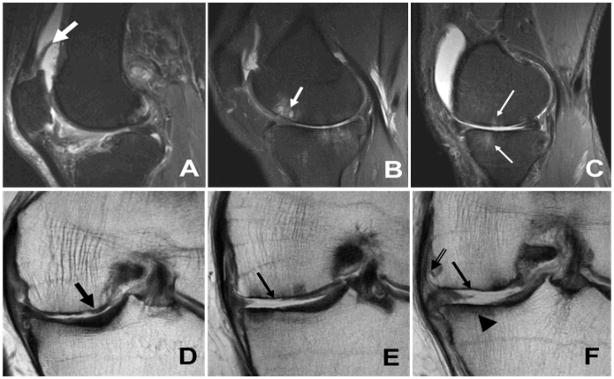
\includegraphics[width=\linewidth]{figs/mud-patologicas-oa.jpg}
    \caption{Imagens de recuperação por inversão sagital (A–C) e eco de spin rápido coronal (D–F) ilustrando os achados da ressonância magnética na osteoartrite. (A) Sinovite reativa (seta branca espessa), (B) Formação de cistos subcondrais (seta branca), (C) Edema da medula óssea (setas brancas finas), (D) Desgaste parcial da cartilagem (seta preta espessa), (E–F) Desgaste total da cartilagem (setas pretas finas), esclerose subcondral (cabeça de seta) e formação de osteófitos marginais (seta dupla). Imagem cortesia dos Drs. Hollis Potter e Catherine Hayter, Hospital for Special Surgery, Nova York, NY. Fonte: \cite{Loeser2012}.}
    \label{fig:osteoartrite-joelho}
\end{figure}

\subsection{Impacto da OA na Qualidade de Vida}

De acordo com o World Health Organization (WHO), "qualidade de vida" é definida como a percepção do indivíduo sobre sua posição de vida no contexto da cultura e sistema de valores que ele vive e em relação aos seus objetivos, expectativas, padrões e preocupações \citep{who2012}.

Existe um grande esforço de pesquisadores e especialistas para avaliar o grau de incapacidade física causado pela doença, além de avaliar os efeitos de diferentes tratamentos em aspectos como dor, função física e mobilidade. No entanto, tais manifestações físicas afetam diretamente outras áreas na vida dos pacientes, como interações sociais, saúde mental e qualidade do sono \citep{Ferrel1992}. Além disso, comparado com outras doenças crônicas, pacientes com doenças muscoesqueléticas, como a OA, são os mais afetados em termos de qualidade de vida. A OA de joelho, especificamente, tende a declinar progressivamente a qualidade de vida conforme a progressão da doença \citep{Hoogeboom2013}.

\cite{Desmeules2009} realizaram um estudo com 197 pacientes com cirurgia agendada para substituição total do joelho (TKA) e avaliaram, através da escala de qualidade de vida SF-36 \citep{Ware1992}, a relação entre a OA de joelho e a qualidade de vida. Os resultados mostraram que a pontuação média da qualidade de vida dos pacientes era significativamente menor do que a população geral no Canadá (p < 0,05). Outros estudos também mostraram resultados similares em pacientes esperando por TKA \citep{Snider2005,Kapetanakis2011}. É razoável, portanto, que pacientes com OA de joelho severa tenham baixos níveis de qualidade de vida comparado com a população geral.

\cite{Sutbeyaz2007} fizeram um estudo com 28 pacientes obesos com OA de joelho e avaliaram a qualidade de vida através da escala de qualidade de vida SF-36. Os resultados mostraram que os pacientes obesos tiveram pontuações muito mais baixas em todos os domínios da escala SF-36, em comparação com o grupo de controle (p < 0,001). Além disso, a obesidade foi associada a uma pior qualidade de vida em pacientes com OA de joelho, o que sugere que a perda de peso pode ser benéfica para melhorar a qualidade de vida desses pacientes.

Complementarmente, \cite{Kawano2015} mostraram que existe uma relação do nível de escolaridade com a capacidade funcional e dor em pacientes com OA de joelho. O estudo foi conduzido com 93 pacientes tratados no Serviço de Ortopedia e Traumatologia do Hospital Santa Izabel e Santa Casa da Misericórdia da Bahia, em Salvador, Brasil. A avaliação da qualidade de vida foi feita através do questionário SF-36 e mostrou que pacientes com níveis mais baixos de escolaridade tiveram pontuações mais baixas nos domínios de capacidade funcional (p < 0,001), limitação funcional (p = 0,009) e dor (p = 0,01), em comparação com pacientes com níveis mais altos de escolaridade (p < 0,05). Além disso, a escolaridade foi associada a uma melhor qualidade de vida em pacientes com OA de joelho, o que sugere que a educação pode ser um fator importante para melhorar a qualidade de vida desses pacientes.

\subsection{Prevalência da OA}

Dados recentes do Global Burden of Disease (GBD) - o estudo epidemiológico observacional mais abrangente do mundo - revelaram que a prevalência da OA cresceu 132\% entre 1990 e 2020, com projeções de crescimento de 60 a 100\% até 2050, alcançando a marca de 1 bilhão de pessoas. Com uma prevalência de 7,6\% da população global em 2020, o que equivale a aproximadamente 595 milhões de pessoas, a OA é mais comum em países desenvolvidos, devido à correlação com o status socieconômico, e contribui significativamente para os chamados "anos vividos com incapacidade" (YLDs em inglês). Além disso, o estudo também aponta que a OA é mais comum em mulheres do que em homens, com prevalência de 8,0\% e 5,8\%, respectivamente, além de atingir principalmente idosos, especialmente aqueles acima de 70 anos, onde a OA assume a 7ª posição entre as principais causas de incapacidade, primeiramente afetando a articulação do joelho \citep{COURTIES20241397}.

No Brasil, \cite{RodriguesSenna2004} realizaram um estudo com mais 3 mil pessoas e identificaram cerca de 7,2\% com doenças reumáticas, sendo a OA a mais comum, com prevalência de 4,14\%. Essa prevalência tende a aumentar visto que, além de existir uma correlação entre a OA e a obesidade, estima-se que o Brasil tenha uma taxa de sobrepeso e obesidade combinados de 68,1\% em 2030 \citep{fiocruz2024}.

% \subsection{Custos associados ao tratamento da OA}
% https://www.scielo.br/j/csp/a/RTcZ4yrgQW3YjpzsF453prQ/?format=pdf&lang=pt
% https://www.scielo.br/j/rbcf/a/9TRjg6CfTgYB9qxSCPgD6Sd/?format=pdf&lang=pt
% https://pmc.ncbi.nlm.nih.gov/articles/PMC8153072/
% https://pmc.ncbi.nlm.nih.gov/articles/PMC4422214/pdf/nihms685605.pdf

\subsection{Diagnóstico e Métodos de Avaliação da OA}

O diagnóstico da OA normalmente é feito com base em exames clínicos, como a avaliação dos sintomas do paciente, exames de imagem, como radiografias e ressonâncias magnéticas, e exames laboratoriais, como a análise do líquido sinovial \citep{Kraus2015}. Exames de raio-x tem sido o método mais comum para diagnosticar a OA, pois é uma abordagem acessível e permite visualizar o espaço articular e alterações ósseas e cartilaginosas nas articulações, como a formação de osteófitos.

Essa avaliação é tipicamente feita por radiologistas a partir de radiografias do joelho extendido ou flexionado, dependendo da necessidade de visualização intra-articular \citep{Braun2012}. A partir dessas imagens, é possível fazer a classificação da severidade da OA e, em caso de diagnótico, recomendar tratamentos farmacêuticos e não farmacêuticos, como exercícios de fortalecimento muscular e fisioterapia.

\subsection{Classificação da OA de Joelhos}

\cite{KELLGREN1957} propuseram uma escala de classificação da OA baseada em radiografias e considerando fatores como a formação de osteófitos, estreitamento da cartilagem articular e esclerose subcondral. A escala de Kellgren/Lawrence (KL) classifica a OA em cinco estágios de progressão: 0 (nenhum), 1 (duvidoso), 2 (mínimo), 3 (moderado) e 4 (grave) (\autoref{tabela-kl}). Como a classificação é comumente feita por radiologistas, estes avaliam as radiografias e atribuem um grau de acordo com a experiência e cuidado médico na interpretação das imagens.

No entanto, a classificação manual pode ser subjetiva e suscetível a erros, assim como foi observado pelos autores, o que pode levar a diagnósticos tardios ou incorretos num cenário onde a detecção precoce é crucial para retardar a progressão da doença, uma vez que não existem medicamentos capazes de retardar o seu desenvolvimento .

\begin{table}[htbp]
    \centering
    \begin{tabular}{|c|c|c|c|c|}
        \hline
        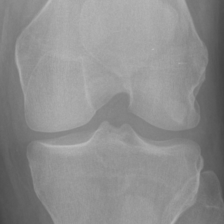
\includegraphics[width=1.7cm]{figs/KL0-sample.png} & 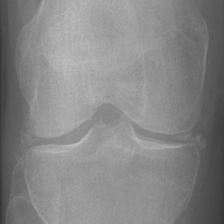
\includegraphics[width=1.7cm]{figs/KL1-sample.png} & 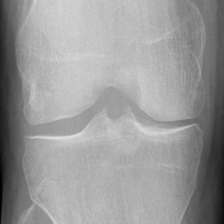
\includegraphics[width=1.7cm]{figs/KL2-sample.png} & 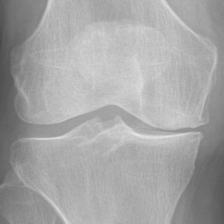
\includegraphics[width=1.7cm]{figs/KL3-sample.png} & 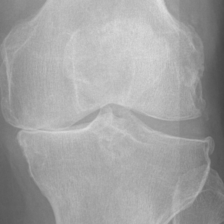
\includegraphics[width=1.7cm]{figs/KL4-sample.png} \\
        \hline
        \textbf{0 (saudável)} & \textbf{1 (duvidoso)} & \textbf{2 (mínimo)} & \textbf{3 (moderado)} & \textbf{4 (severo)} \\
        \hline
    \end{tabular}
    \caption{Escala de Kellgren/Lawrence para classificação da severidade de osteoartrite.}
    \label{tabela-kl}
\end{table}

\section{Rede Neural Convolucional (RNC)}\label{sec:rnc}

Uma rede neural artificial é um modelo computacional inspirado no cérebro humano \citep{McCulloch1943}, onde neurônios artificiais recebem um conjunto de entradas ponderadas, realizam uma soma dessas entradas e aplicam uma função de ativação para produzir uma saída. Essa estrutura permite que as redes neurais aprendam padrões complexos a partir de dados, tornando-as adequadas para tarefas de processamento de linguagem natural, visão computacional, entre outras aplicações.

Em 2006, \cite{Hinton2006} propuseram o uso de redes neurais artificiais com múltiplas camadas com o objetivo de melhorar a capacidade dos modelos, o que levou a um renascimento do interesse nessas redes e ao desenvolvimento de novas arquiteturas, como é o caso da rede neural convolucional (CNN, do inglês \textit{Convolutional Neural Network}).

As CNNs são modelos de aprendizado profundo projetados para processar dados com estrutura de grade, como imagens. Inspiradas na organização do córtex visual, CNNs são amplamente utilizadas em tarefas de visão computacional, como classificação de imagens, detecção de objetos e segmentação semântica.

A camada de convolução é o componente central das CNNs, responsável por extrair características locais dos dados de entrada. Essa camada utiliza filtros (ou \textit{kernels}), que são pequenas matrizes de pesos (por exemplo, 3x3 ou 5x5) aplicadas em toda a imagem de entrada para gerar um mapa de características (ou \textit{feature maps}), representando a presença dessas características em diferentes regiões da imagem.

Esses filtros são ajustados durante o treinamento da rede, permitindo que a CNN aprenda a detectar padrões relevantes, como bordas, texturas e formas. Conforme a rede avança pelas camadas, os filtros se tornam mais complexos e capazes de capturar características de alto nível, como objetos inteiros. Após as convoluções, é comum utilizar a função de ativação ReLU (\textit{Rectified Linear Unit}), que substitui valores negativos por zero e introduz não linearidades no modelo, permitindo que ele aprenda representações complexas.

Após as camadas de convolução, as CNNs geralmente incluem camadas de \textit{pooling} para reduzir a dimensionalidade dos \textit{feature maps}, enquanto preservam as características mais relevantes. O \textit{pooling} pode ser feito de várias maneiras, como \textit{max pooling} (onde o valor máximo de uma região é mantido) ou \textit{average pooling} (onde a média dos valores é calculada). Esse processo contribui para:

\begin{itemize}
    \item reduzir a quantidade de parâmetros e o custo computacional da rede.
    \item tornar a rede mais robusta a pequenas variações nos dados de entrada.
\end{itemize}

Após diversas camadas de convolução e \textit{pooling}, uma ou mais camadas totalmente conectadas (\textit{fully connected}) são adicionadas ao final da rede para combinar as características extraídas de camadas anteriores e realizar a tarefa de classificação. Cada neurônio dessas camadas está conectado a todos os valores da camada anterior, permitindo decisões baseadas em combinações globais das informações aprendidas. Em tarefas de classificação, a última camada totalmente conectada geralmente utiliza a função de ativação \textit{softmax}, que transforma as saídas em probabilidades.

Durante o treinamento, a CNN ajusta os pesos dos filtros por meio do algoritmo de retropropagação (\textit{backpropagation}), em que o erro de saída é retropropagado pela rede para atualizar os pesos e minimizar a função de perda. Esse processo é repetido por várias épocas, permitindo que a rede aprenda a reconhecer padrões complexos nos dados de entrada.

A \autoref{fig:cnn} ilustra uma rede neural convolucional composta por cinco camadas. O número de camadas, a disposição dessas camadas, o número e tamanho dos filtros, a forma de conexão entre as camadas, entre outros fatores, podem variar dependendo da arquitetura escolhida. Em seguida, serão aprensentadas algumas das arquiteturas populares de CNN que serão utilizadas neste trabalho.

\begin{figure}
    \centering
    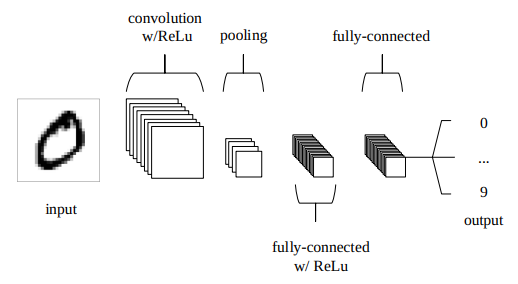
\includegraphics[width=0.5\linewidth]{figs/convolution-neural-network.png}
    \caption{Uma rede neural convolucional simples, composta por apenas cinco camadas. Fonte: \cite{Saxena2022}.}
    \label{fig:cnn}
\end{figure}

\subsection{VGG (Visual Geometry Group Network)}

Os modelos VGG foram introduzidos pelo \textit{Visual Geometry Group} da Universidade de Oxford por \cite{Simonyan2015}, que depois serviu como base para a competição do \textit{ImageNet} em 2014, quando conquistaram o primeiro e segundo lugar na época. A arquitetura VGG é conhecida por sua simplicidade e profundidade, utilizando filtros convolucionais pequenos (3×3) empilhados em camadas profundas, variando de 11 a 19 camadas. O objetivo dos autores era explorar o impacto da profundidade na performance do modelo, e eles descobriram que redes neurais mais profundas superavam redes mais rasas, desde que treinadas adequadamente.

A arquitetura VGG processa imagens RGB de 224×224 pixels, utilizando uma série de camadas convolucionais seguidas por camadas de \textit{pooling}, onde cada camada contém um número crescente de filtros 3×3. O \textit{stride} é fixo em 1 pixel, e o \textit{padding} é utilizado para manter a dimensão da imagem. Após as camadas convolucionais, são aplicadas camadas de \textit{max-pooling} com um tamanho de 2×2 e \textit{stride} de 2, reduzindo a dimensão da imagem pela metade. Por fim, são adicionadas três camadas totalmente conectadas (ou \textit{fully connected} do inglês), seguidas por uma camada de saída com ativação \textit{softmax} para classificação. Além disso, as camadas escondidas são ativadas por funções ReLU, reponsáveis por introduzir a não-linearidade no modelo.

A tabela \ref{vgg-arch} apresenta a configuração das arquiteturas VGG-16 e VGG-19, com um total de 16 e 19 camadas, respectivamente. Ambas se destacaram na competição do \textit{ImageNet} e são amplamente utilizadas devido à sua performance em tarefas de classificação, incluindo o diagnóstico a partir de imagens médicas \citep{Saini2023, Sitaula2021}. Por esse motivo, estas arquiteturas serão utilizadas nesta pesquisa como comparação com os demais modelos.

\begin{table}[h]
    \centering
    \footnotesize
    \begin{tabular}{|c|c|}
        \hline
        \textbf{VGG-16} & \textbf{VGG-19} \\
        \hline
        16 camadas & 19 camadas \\
        \hline
        \multicolumn{2}{|c|}{imagem RGB de entrada (224 x 224)} \\
        \hline
        conv3-64 & conv3-64 \\
        conv3-64 & conv3-64 \\
        \hline
        \multicolumn{2}{|c|}{maxpool} \\
        \hline
        conv3-128 & conv3-128 \\
        conv3-128 & conv3-128 \\
        \hline
        \multicolumn{2}{|c|}{maxpool} \\
        \hline
        conv3-256 & conv3-256 \\
        conv3-256 & conv3-256 \\
        conv3-256 & conv3-256 \\
         & \textbf{conv3-256} \\
        \hline
        \multicolumn{2}{|c|}{maxpool} \\
        \hline
        conv3-512 & conv3-512 \\
        conv3-512 & conv3-512 \\
        conv3-512 & conv3-512 \\
         & \textbf{conv3-512} \\
        \hline
        \multicolumn{2}{|c|}{maxpool} \\
        \hline
        conv3-512 & conv3-512 \\
        conv3-512 & conv3-512 \\
        conv3-512 & conv3-512 \\
         & \textbf{conv3-512} \\
        \hline
        \multicolumn{2}{|c|}{maxpool} \\
        \hline
        \multicolumn{2}{|c|}{FC-4096} \\
        \hline
        \multicolumn{2}{|c|}{FC-4096} \\
        \hline
        \multicolumn{2}{|c|}{FC-1000} \\
        \hline
        \multicolumn{2}{|c|}{softmax} \\
        \hline
    \end{tabular}
    \caption{Configuração dos modelos VGG-16 e VGG-19. Os parâmetros de cada camada convolucional são denotados por "conv<tamanho do campo receptivo>-<número de canais>". A função de ativação ReLU não é exibida por motivos de simplicidade.}
    \label{vgg-arch}
\end{table}

\subsection{ResNet (Residual Network)}

\cite{He2016} venceram a competição ILSVRC 2015 com a arquitetura \textit{Residual Network} (\textit{ResNet}), que introduziu a ideia de blocos residuais e alcançou uma taxa de erro de 3,57\% no conjunto de validação do \textit{ImageNet} com um \textit{ensemble} de seus modelos. Os autores abordaram o problema da degradação de desempenho: conforme a profundidade da rede aumentava, a acurácia saturava e começava a diminuir. Para resolver, eles introduziram a ideia de conexões de atalho (\textit{skip connections}) entre as camadas, onde o sinal de entrada de uma camada é somado ao sinal de saída de uma camada subsequente (\autoref{residual-learning}).

Formalmente, considerando que o objetivo de uma rede neural é aprender uma função \( H(x) \), onde \( x \) é a entrada, a ResNet propõe que a rede aprenda uma função residual \( F(x) = H(x) - x \), onde a entrada \( x \) é adicionada à saída \( H(x) \), reformulando a função de aprendizado como \( H(x) = F(x) + x \). Essa abordagem permite que a rede aprenda funções de identidade mais facilmente, facilitando o treinamento de redes mais profundas sem adicionar complexidade.

\begin{figure}[h]
    \centering
    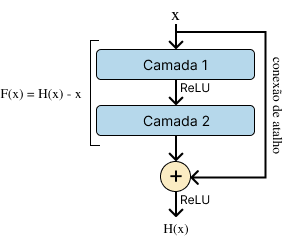
\includegraphics[width=0.5\linewidth]{figs/residual-connection.png}
    \caption{Aprendizado residual}
    \label{residual-learning}
\end{figure}

A arquitetura ResNet é composta por pilhas de blocos residuais que consistem em duas camadas convolucionais, com um \textit{Batch Normalization} e uma função de ativação ReLU entre elas. As camadas convolucionais utilizam filtros de tamanho 3×3, com um \textit{stride} de 1 e \textit{padding} de 1, para manter a dimensão da imagem. A saída do bloco residual é então somada à entrada original, permitindo que o modelo aprenda a função residual. A rede termina com uma camada de \textit{average pooling} global e uma camada totalmente conectada (ou \textit{fully connected} do inglês) com ativação \textit{softmax} para classificação.

A tabela \ref{resnet-arch} apresenta a configuração das arquiteturas ResNet-34, ResNet-50 e ResNet-101, que são variantes da ResNet com diferentes profundidades. Essas arquiteturas foram escolhidas devido à sua popularidade e eficácia em tarefas de classificação de imagens, especialmente em radiografias. \cite{Leung2020} utilizaram a arquitetura ResNet-34 para diagnosticar a OA de joelhos em pacientes submetidos à artroplastia total do joelho (TKA) e obtiveram resultados que superaram modelos de resultados binários.

\begin{table}[h]
    \centering
    \footnotesize
    \begin{tabular}{|c|c|c|c|c|}
        \hline
        \textbf{Camada} & \textbf{Tamanho da saída} & \textbf{34 camadas} & \textbf{50 camadas} & \textbf{101 camadas} \\
        \hline
        conv1 & 112×112 & \multicolumn{3}{c|}{7×7, 64, stride 2} \\
        \hline
        \multicolumn{2}{|c|}{ } & \multicolumn{3}{c|}{3×3 max pool, stride 2} \\
        \hline
        conv2\_x & 56×56 & 
        $\left[\begin{array}{c}
        3 \times 3, 64 \\
        3 \times 3, 64
        \end{array}\right] \times 3$ & 
        $\left[\begin{array}{c}
        1 \times 1, 64 \\
        3 \times 3, 64 \\
        1 \times 1, 256
        \end{array}\right] \times 3$ & 
        $\left[\begin{array}{c}
        1 \times 1, 64 \\
        3 \times 3, 64 \\
        1 \times 1, 256
        \end{array}\right] \times 3$ \\
        \hline
        conv3\_x & 28×28 &
        $\left[\begin{array}{c}
        3 \times 3, 128 \\
        3 \times 3, 128
        \end{array}\right] \times 4$ & 
        $\left[\begin{array}{c}
        1 \times 1, 128 \\
        3 \times 3, 128 \\
        1 \times 1, 512
        \end{array}\right] \times 4$ & 
        $\left[\begin{array}{c}
        1 \times 1, 128 \\
        3 \times 3, 128 \\
        1 \times 1, 512
        \end{array}\right] \times 4$ \\
        \hline
        conv4\_x & 14×14 & 
        $\left[\begin{array}{c}
        3 \times 3, 256 \\
        3 \times 3, 256
        \end{array}\right] \times 6$ & 
        $\left[\begin{array}{c}
        1 \times 1, 256 \\
        3 \times 3, 256 \\
        1 \times 1, 1024
        \end{array}\right] \times 6$ & 
        $\left[\begin{array}{c}
        1 \times 1, 256 \\
        3 \times 3, 256 \\
        1 \times 1, 1024
        \end{array}\right] \times 23$ \\
        \hline
        conv5\_x & 7×7 &
        $\left[\begin{array}{c}
        3 \times 3, 512 \\
        3 \times 3, 512
        \end{array}\right] \times 3$ &
        $\left[\begin{array}{c}
        1 \times 1, 512 \\
        3 \times 3, 512 \\
        1 \times 1, 2048
        \end{array}\right] \times 3$ & 
        $\left[\begin{array}{c}
        1 \times 1, 512 \\
        3 \times 3, 512 \\
        1 \times 1, 2048
        \end{array}\right] \times 3$ \\
        \hline
         & 1×1 & \multicolumn{3}{c|}{average pool, 1000-d fc, softmax} \\
        \hline
        \multicolumn{2}{|c|}{FLOPs} & 3.6×10\textsuperscript{9} & 3.8×10\textsuperscript{9} & 7.6×10\textsuperscript{9} \\
        \hline
    \end{tabular}
    \caption{Configuração das arquiteturas ResNet-34, ResNet-50 e ResNet-101.}
    \label{resnet-arch}
\end{table}

\subsection{DenseNet (Densely Connected Convolutional Networks)}

A arquitetura DenseNet introduziu uma nova abordagem para lidar com redes profundas e aliviar o problema de \textit{vanishing gradients}, melhorando a propagação e reuso da informação, além de diminuir o número de parâmetros. A ideia principal foi conectar cada camada a todas as camadas anteriores, formando conexões densas entre elas. Isso significa que cada camada recebe como entrada não apenas a saída da camada anterior, mas também as saídas de todas as camadas anteriores (\autoref{dense-network}). Essa abordagem permite que o modelo aprenda representações mais ricas e complexas, facilitando a extração de características relevantes para a tarefa de classificação \citep{Huang2017}.

\begin{figure}[h]
    \centering
    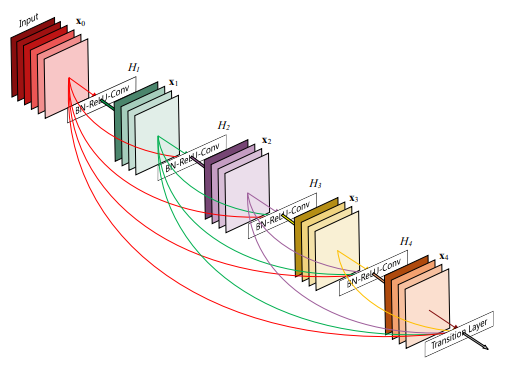
\includegraphics[width=0.5\linewidth]{figs/dense-network.png}
    \caption{Um bloco de 5 camadas de uma DenseNet. Cada camada recebe como entrada a saída de todas as camadas anteriores.}
    \label{dense-network}
\end{figure}

O componente fundamental da DenseNet é o bloco denso (ou \textit{dense block} em inglês), que consiste em várias camadas convolucionais conectadas densamente. Cada camada dentro do bloco denso aplica três operações consecutivas: \textit{batch normalization} (BN), seguido de uma função de ativação ReLU e, por fim, uma convolução 3×3. Após a aplicação do bloco denso, uma transição (ou \textit{transition} em inglês) é realizada para reduzir a dimensão dos \textit{feature maps} usando uma camada de convolução 1×1, seguida por uma camada de \textit{average pooling} 2×2.

Portanto, a arquitetura DenseNet é composta por quatro blocos densos, cada um seguido por camadas de transição. A saída final (classificador) é obtida através de uma camada de \textit{global average pooling} e uma camada totalmente conectada com ativação \textit{softmax} para classificação. A tabela \ref{densenet-arch} apresenta a configuração das arquiteturas DenseNet-121 e DenseNet-169, que são variantes da DenseNet com diferentes profundidades que serão utilizadas neste trabalho, pois fornecem um bom equilíbrio entre complexidade e desempenho comparado com outras arquiteturas mais profundas.

Nos últimos anos, as arquiteturas DenseNet têm sido amplamente utilizadas em diversas tarefas de classificação de imagens, incluindo diagnósticos médicos. Por exemplo, \citep{Rajpurkar2017} propuseram um modelo chamado CheXNet baseado na arquitetura DenseNet-121 para detectar pneumonia a partir de radiografias torácicas, superando o desempenho médio de radiologistas na métrica F1-score.

\begin{table}[h]
    \centering
    \footnotesize
    \begin{tabular}{|c|c|c|c|}
        \hline
        \textbf{Camadas} & \textbf{Tamanho da saída} & \textbf{DenseNet-121} & \textbf{DenseNet-169} \\
        \hline
        Convolução & 112×112 & \multicolumn{2}{c|}{7×7 conv, stride 2} \\
        \hline
        Pooling & 56×56 & \multicolumn{2}{c|}{3×3 max pool, stride 2} \\
        \hline
        Dense Block (1) & 56×56 & 
        $\left[\begin{array}{c}
        1 \times 3 \\
        3 \times 3
        \end{array}\right] \times 6$ & 
        $\left[\begin{array}{c}
        1 \times 3 \\
        3 \times 3
        \end{array}\right] \times 6$ \\
        \hline
        \multirow{2}{*}{Transition Layer (1)} & 56×56 & \multicolumn{2}{c|}{$1 \times 1$ conv} \\
        \cline{2-4}
        & 28×28 & \multicolumn{2}{c|}{$2 \times 2$ average pool, stride 2} \\
        \hline
        Dense Block (2) & 28×28 & 
        $\left[\begin{array}{c}
        1 \times 3 \\
        3 \times 3
        \end{array}\right] \times 12$ & 
        $\left[\begin{array}{c}
        1 \times 3 \\
        3 \times 3
        \end{array}\right] \times 12$ \\
        \hline
        \multirow{2}{*}{Transition Layer (2)} & 28×28 & \multicolumn{2}{c|}{$1 \times 1$ conv} \\
        \cline{2-4}
        & 14×14 & \multicolumn{2}{c|}{$2 \times 2$ average pool, stride 2} \\
        \hline
        Dense Block (3) & 14×14 & 
        $\left[\begin{array}{c}
        1 \times 3 \\
        3 \times 3
        \end{array}\right] \times 24$ & 
        $\left[\begin{array}{c}
        1 \times 3 \\
        3 \times 3
        \end{array}\right] \times 32$ \\
        \hline
        \multirow{2}{*}{Transition Layer (3)} & 14×14 & \multicolumn{2}{c|}{$1 \times 1$ conv} \\
        \cline{2-4}
        & 7×7 & \multicolumn{2}{c|}{$2 \times 2$ average pool, stride 2} \\
        \hline
        Dense Block (4) & 7×7 & 
        $\left[\begin{array}{c}
        1 \times 3 \\
        3 \times 3
        \end{array}\right] \times 16$ & 
        $\left[\begin{array}{c}
        1 \times 3 \\
        3 \times 3
        \end{array}\right] \times 32$ \\
        \hline
        \multirow{2}{*}{Classification Layer} & 1×1 & \multicolumn{2}{c|}{$7 \times 7$ global average pool} \\
        \cline{2-4}
        &  & \multicolumn{2}{c|}{1000D fully-connected, softmax} \\
        \hline
    \end{tabular}
    \caption{Configuração das arquiteturas DenseNet-121 e DenseNet-169.}
    \label{densenet-arch}
\end{table}

\subsection{Inception-v3}

A arquitetura Inception, introduzida por \cite{Szegedy2015} no contexto do desafio ILSVRC 2014, representou um avanço significativo na evolução das redes neurais convolucionais. Seu principal diferencial está na proposta de uma estrutura modular - o módulo Inception - que combina convoluções de diferentes tamanhos (1×1, 3×3, 5×5) e operações de \textit{pooling} em paralelo, promovendo o processamento de informações em múltiplas escalas (\autoref{inception-module}).

O modelo GoogLeNet, uma instância da arquitetura Inception com 22 camadas profundas, obteve o primeiro lugar no ILSVRC 2014 \citep{Russakovsky2015}, alcançando um notável desempenho em tarefas de classificação e detecção, mesmo utilizando significativamente menos parâmetros que modelos anteriores, como o VGG.

\begin{figure}[h]
    \centering
    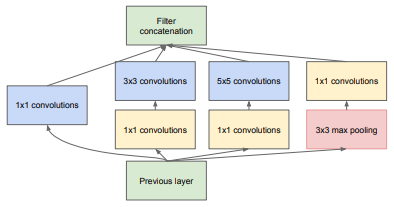
\includegraphics[width=0.5\linewidth]{figs/inception-module.png}
    \caption{Um módulo Inception.}
    \label{inception-module}
\end{figure}

A arquitetura Inception-v3 \citep{Szegedy2016} representa uma evolução significativa em relação ao modelo original Inception (GoogLeNet), incorporando diversas inovações voltadas à melhoria da eficiência computacional e da acurácia. Entre as principais contribuições estão a fatoração de convoluções em operações menores e assimétricas (\autoref{inception-module-v3}), o uso mais sistemático da normalização em lote (\textit{batch normalization}) e a adoção da técnica de \textit{label smoothing} como forma de regularização. Tais aprimoramentos resultaram em um modelo mais profundo e preciso, mantendo um custo computacional viável para aplicações práticas.

\begin{figure}[h]
    \centering
    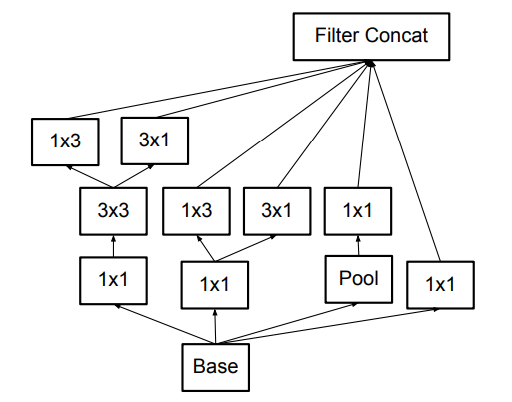
\includegraphics[width=0.5\linewidth]{figs/inception-module-v3.png}
    \caption{Um módulo Inception com fatoração de convoluções.}
    \label{inception-module-v3}
\end{figure}

A \autoref{inception-v3-arch} apresenta a configuração da arquitetura Inception-v3, com um total de 42 camadas, que inclui a fatoração de convoluções tradicionais 7×7 em convoluções 3×3. A arquitetura substitui o otimizador padrão do SGD por um otimizador mais avançado, o RMSProp, favorecendo a convergência do modelo durante o treinamento, além de utilizar classificadores auxiliares com normalização em lote nas camadas intermediárias, melhorando a propagação do sinal do gradiente e, por consequência, a eficiência do treinamento.

\begin{table}[ht]
    \centering
    \footnotesize
    \begin{tabular}{|l|c|c|c|c|}
        \hline
        \textbf{type} & \textbf{patch size/stride} & \textbf{input size} \\
        \hline
        conv & $3\times3$/2 & $299\times299\times3$ \\
        \hline
        conv & $3\times3$/1 & $149\times149\times32$ \\
        \hline
        conv padded & $3\times3$/1 & $147\times147\times32$ \\
        \hline
        pool & $3\times3$/2 & $147\times147\times64$ \\
        \hline
        conv & $3\times3$/1 & $73\times73\times64$ \\
        \hline
        conv & $3\times3$/2 & $71\times71\times80$ \\
        \hline
        conv & $3\times3$/1 & $35\times35\times192$ \\
        \hline
        $3\times$Inception &  & $35\times35\times288$ \\
        \hline
        $5\times$Inception &  & $17\times17\times768$ \\
        \hline
        $2\times$Inception &  & $8\times8\times1280$ \\
        \hline
        pool & $8\times8$ & $8\times8\times2048$ \\
        \hline
        linear & logits & $1\times1\times2048$ \\
        \hline
        softmax & classifier & $1\times1\times1000$ \\
        \hline
    \end{tabular}
    \caption{Configuração da arquitetura Inception-v3.}
    \label{inception-v3-arch}
\end{table}

Além de seu excelente desempenho na tarefa de classificação de imagens do ILSVRC 2012 \citep{Russakovsky2015}, a arquitetura Inception-v3 tem sido utilizada em outras aplicações, incluindo o diagnóstico médico. Por exemplo, \cite{Mujahid2022} adotaram a arquitetura Inception-v3 para a tarefa de classificação de pneumonia em radiografias e obtiveram resultados promissores, alcançando uma acurácia de 99,29\% com um ensemble, superando outros modelos, como VGG-16 e ResNet-50.

\subsection{Aprendizado por Transferência}

O aprendizado por transferência \citep{Zhuang2021} é uma técnica de aprendizado de máquina no qual o conhecimento adquirido por um modelo treinado em uma tarefa é reutilizado para solucionar outra tarefa relacionada, mas diferente. Essa abordagem é especialmente útil para evitar o treinamento de modelos do zero, economizando tempo e recursos computacionais, além de melhorar o desempenho em tarefas com poucos dados disponíveis.

Em redes neurais, o aprendizado por transferência é frequentemente realizado reutilizando pesos de um modelo pré-treinado, cujos estágios iniciais da rede geralmente capturam características genéricas das entradas, como bordas ou texturas, que podem ser úteis para resolver novos problemas. Por exemplo, redes neurais treinadas em grandes conjuntos de dados, como o ImageNet \citep{Russakovsky2015}, podem ser reaproveitadas para resolver tarefas específicas, como a classificação de imagens médicas.

Essa estratégia é realizada através do ajuste fino (\textit{fine-tuning} do inglês) do modelo pré-treinado em duas etapas principais. Na primeira, caso seja necessário, as camadas finais do modelo são substituídas por novas camadas adaptadas à tarefa-alvo, como uma camada totalmente conectada com o número de classes correspondente. Na segunda etapa, parte ou toda a rede é treinada com os novos dados. As camadas iniciais geralmente são mantidas inalteradas, enquanto as camadas finais são ajustadas para aprender as características específicas da nova tarefa.

Aplicações de visão computacional e processamento de linguagem natural têm se beneficiado da transferência de aprendizado. Ao reduzir a necessidade de grandes volumes de dados e de poder computacional, essa técnica torna-se uma alternativa viável e eficiente para o desenvolvimento de soluções baseadas em redes neurais profundas.

\section{Visão Computacional}\label{sec:visao-computacional}

A visão computacional é um campo da inteligência artificial (IA) e da ciência da computação (\autoref{definicao-cv}) que estuda como as máquinas podem adquirir, processar, analisar e compreender imagens e vídeos do mundo real, com o objetivo de produzir representações visuais ou descrever o conteúdo visual de forma automática \cite{huggingface2024}.

\begin{figure}[h]
    \centering
    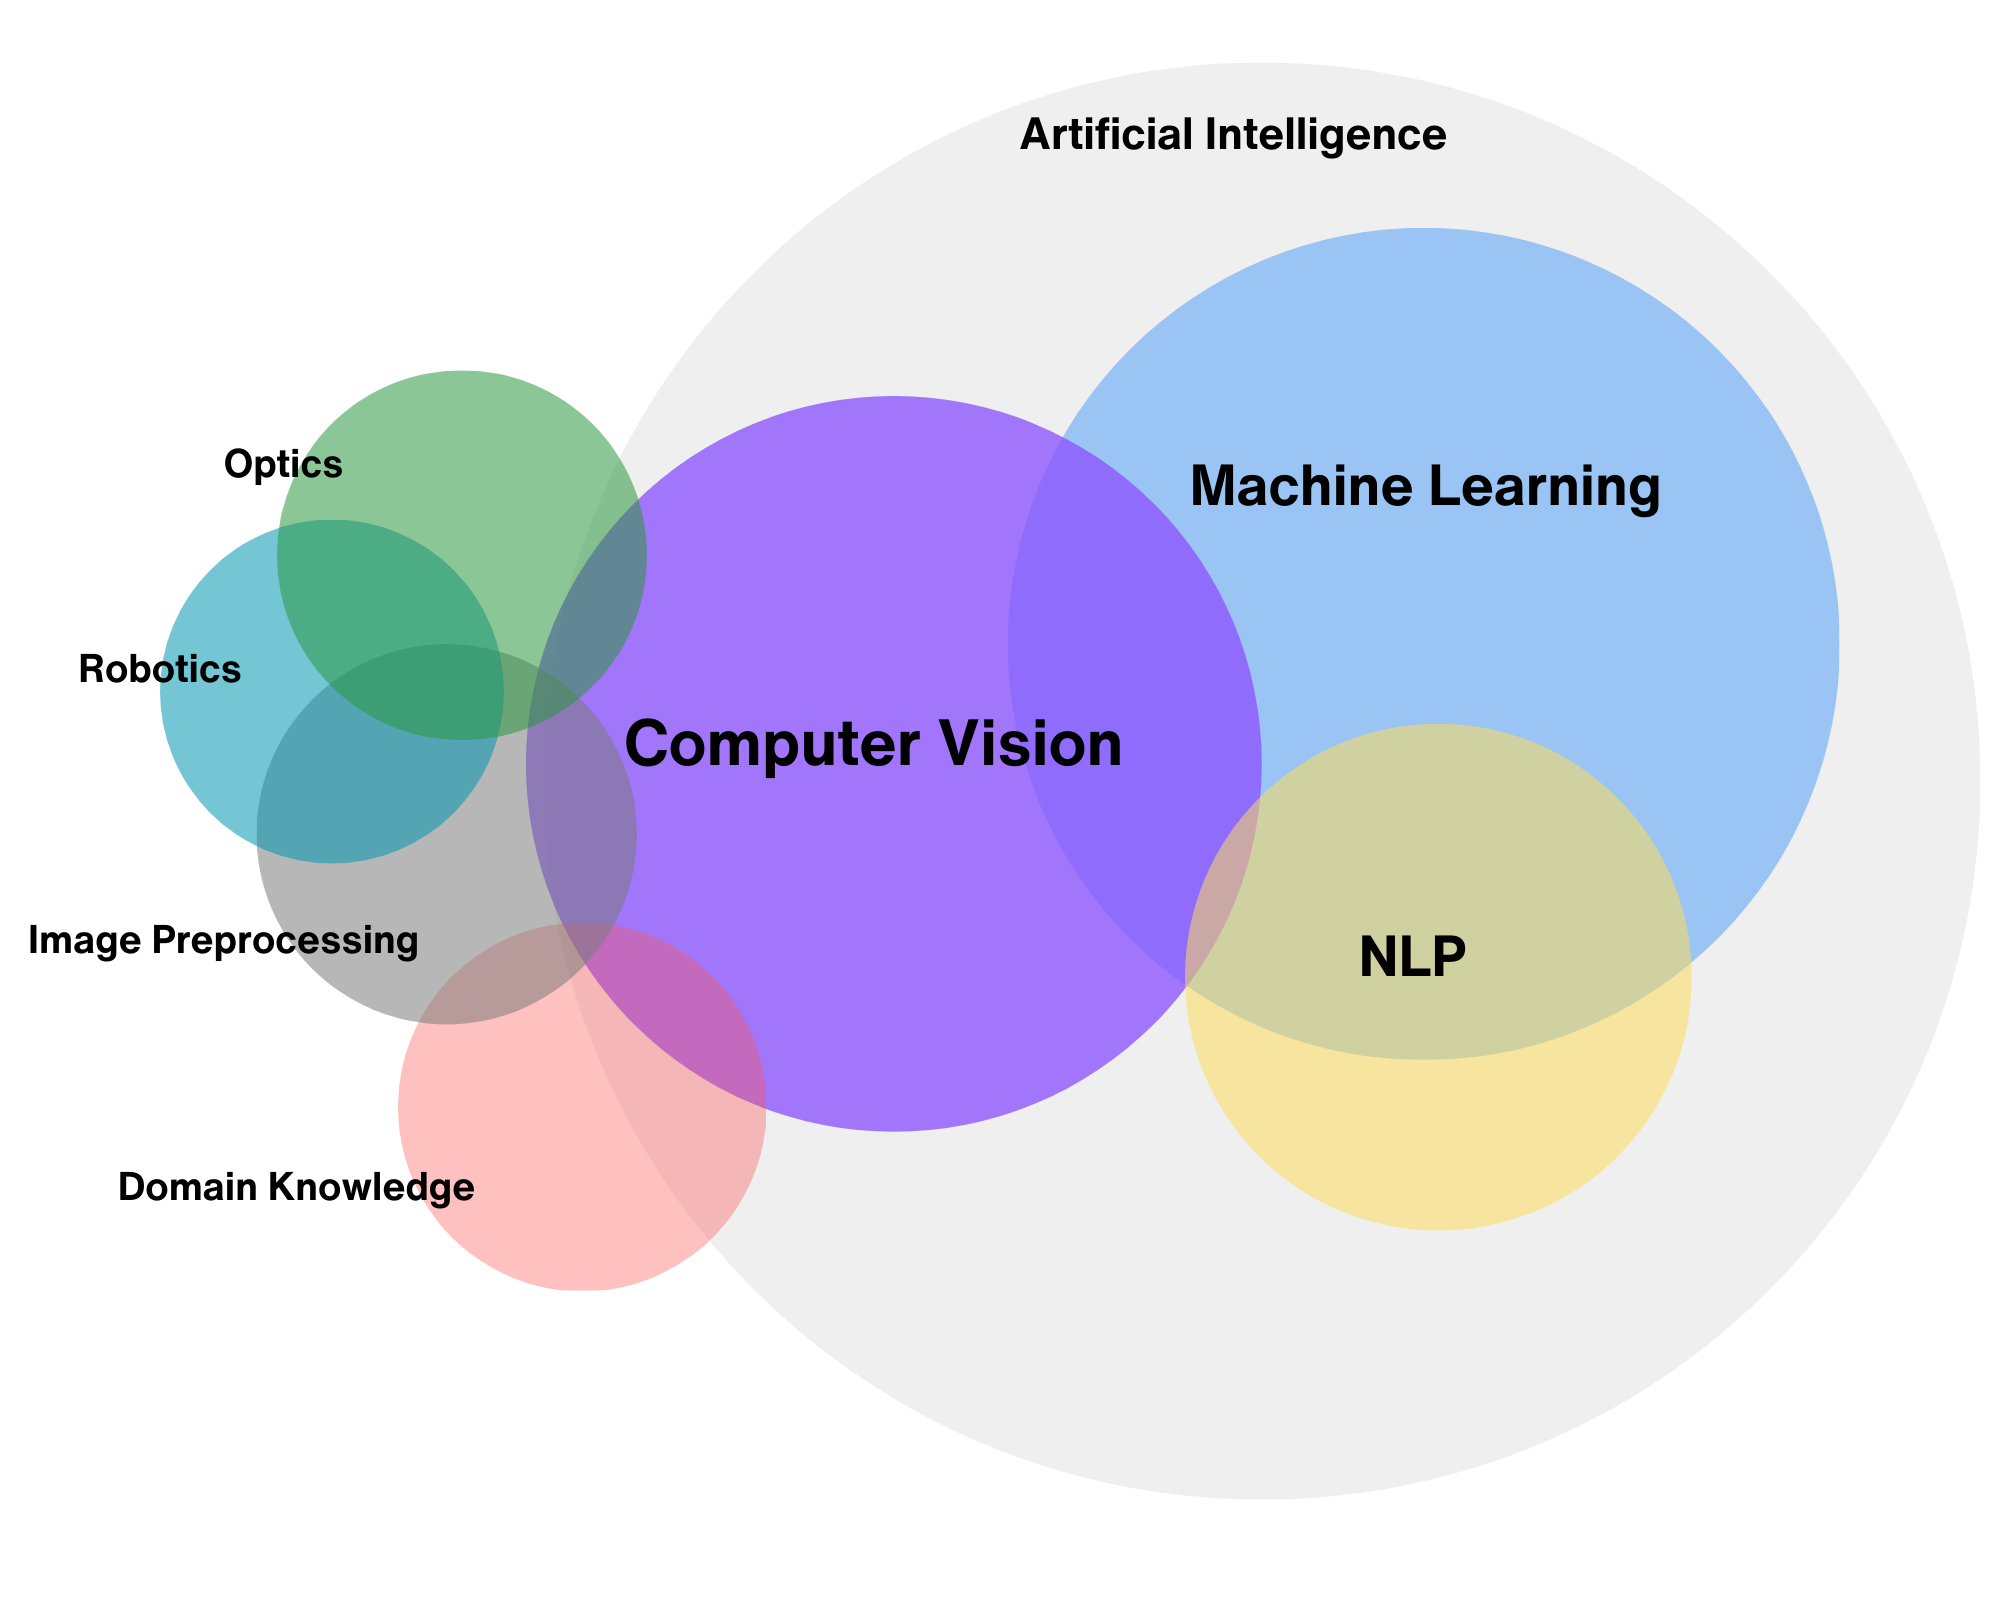
\includegraphics[width=\linewidth]{figs/CV_in_defintiion.png}
    \caption{Definição de visão computacional. Fonte: \cite{huggingface2024}.}
    \label{definicao-cv}
\end{figure}

Essa tecnologia tem se beneficiado de avanços significativos das últimas décadas, incluindo o desenvolvimento e aperfeiçoamento de algoritmos de aprendizado profundo, que permitem a extração de características complexas e abstratas de imagens e vídeos, o aumento da capacidade computacional com o uso de GPUs (Graphics Processing Units), e o desenvolvimento de grandes conjuntos de dados, como o ImageNet, que contém milhões de imagens rotuladas em centenas de categorias \cite{Esteva2021}.

O aprendizado profundo revolucionou a forma como sistemas computacionais processam dados brutos. Tradicionalmente, a construção de modelos exigia conhecimento especializado para extrair manualmente características relevantes dos dados, como bordas, texturas e formas. Enquanto isso, o aprendizado profundo permite que redes neurais descubram automaticamente essas representações em vários níveis de abstração. Esse avanço tem levado a conquistas notáveis em diversas áreas, como reconhecimento de fala, processamento de linguagem natural (PLN) e visão computacional [https://www.cs.toronto.edu/~hinton/absps/NatureDeepReview.pdf].

Em 1963, Larry Roberts, um dos pioneiros da visão computacional, propôs métodos capazes de compreender objetos em 3D a partir de imagens 2D, representando o marco inicial da área [Machine Perception of Thre Dimensional Solids]. Na próxima década, nos anos 1970 e 1980, pesquisadores desenvolveram algoritmos para detectar bordas e cantos em imagens, modelagem poliédrica e não poliédrica, representação de objetos como interconexões de estruturas menores, fluxo óptico e estimativa de movimento [computer vision: algorithms and applications]. Além disso, a década de 1980 foi marcada pela publicação do artigo "Learning representations by back-propagating errors" de David Rumelhart, Geoffrey Hinton e Ronald Williams, que introduziu o algoritmo de retropropagação, que é amplamente utilizado em modelos de aprendizado profundo até hoje [NatureDeepReview, Learning representations by back-propagating errors].

No entanto, foi apenas na decada de 2010 que o aprendizado profundo se tornou popular, com o desenvolvimento de arquiteturas de redes neurais profundas, como as redes neurais convolucionais (CNNs) e as redes neurais recorrentes (RNNs), amplamente adotadas pela comunidade de visão computacional [https://www.cs.toronto.edu/~hinton/absps/NatureDeepReview.pdf]. Em 2012, a equipe de Geoffrey Hinton, chamada de Super Vision, venceu a competição ImageNet Large Scale Visual Recognition Challenge (ILSVRC) com a rede neural convolucional AlexNet, que alcançou resultados significativamente melhores do que os métodos tradicionais de visão computacional em tarefas de classificação e detecção de objetos em imagens [https://arxiv.org/pdf/1409.0575]. Esse avanço marcou a início da era do aprendizado profundo na visão computacional, permitindo a crição de modelos mais sofisticados e precisos, capazes de superar a capacidade humana em tarefas visuais.

Paralelamente, houve uma evolução significativa em hardware computacional, com o desenvolvimento de GPUs, que permitiu treinar modelos de aprendizado profundo em grandes conjuntos de dados de forma mais rápida e eficiente. As GPUs, inicialmente projetadas para renderização de gráficos em jogos e aplicações de design, foram adaptadas para acelerar cálculos matriciais e aplicações computacionalmente intensivas, incluindo o treinamento de redes neurais profundas, devido à sua capacidade de processar informação em paralelo [High performance convolutional neural networks for document processing, Forecasting GPU Performance for Deep Learning Training and Inference]. Em 2009, a equipe de Andrew Ng, da Universidade de Stanford, demonstrou que o uso de GPUs acelerou o treinamento de redes neurais profundas em 70 vezes em comparação com CPUs multi-core, o que permitiu a criação de modelos mais complexos em menos tempo [Large-scale Deep Unsupervised Learning using Graphics Processors]. A partir de então, GPUs se tornaram uma ferramenta essencial para pesquisadores e instituições que trabalham com aprendizado profundo, trazendo mais agilidade e eficiência para o treinamento de modelos.

Apesar dos avanços em algoritmos de aprendizado profundo e hardware computacional, a visão computacional ainda enfrentava desafios quanto à falta de grandes conjuntos de dados rotulados para treinar os modelos de visão computacional. No entanto, em 2009 foi introduzido o ImageNet, um conjunto de dados com milhões de imagens em centenas de categorias, construído sobre a base de dados WordNet, que contém sinônimos e relações semânticas entre palavras. Com isso, o ImageNet se tornou o maior e mais diverso conjunto de dados de imagens disponível na época [ImageNet: A Large-Scale Hierarchical Image Database]. Mais tarde, em 2012, o ImageNet serviu como base para o ImageNet Large Scale Visual Recognition Challenge (ILSVRC), uma competição anual que avalia algoritmos de classificação e detecção de objetos em larga escala. O desafio foi marcado pela vitória da equipe de Geoffrey Hinton, onde propuseram a rede neural convolucional profunda chamada AlexNet capaz de alcançar altas taxas de acurácia e redução significativa na taxa de erro, marcando assim o início da era do aprendizado profundo e solidificando o papel do ImageNet como catalisador para inovações subsequentes na área [ImageNet Large Scale Visual Recognition Challenge].

[tecnicas da visao computacional]

[aplicacoes gerais]

\section{Visão Computacional na Saúde}\label{sec:visao-computacional-saude}

No setor da saúde, a visão computacional tem desempenhado um papel crucial na automação de tarefas clínicas, diagnóstico de doenças, monitoramento de pacientes e tratamentos médicos. A análise de imagens médicas, como radiografias, tomografias, ressonâncias magnéticas e ultrassonografias, é uma das principais aplicações da visão computacional na saúde. A partir dessas imagens, é possível detectar e classificar patologias, monitorar o progresso de doenças, avaliar a eficácia de tratamentos e até mesmo recomendar tratamentos personalizados para pacientes. Além disso, a visão computacional também tem sido utilizada para automatizar tarefas clínicas, como a identificação de pacientes, a análise de exames laboratoriais e a triagem de pacientes em hospitais e clínicas \cite{JAVAID2024792}.

Na área da saúde, a visão computacional tem sido muito utilizada para melhorar a acurácia de diagnósticos, automatização de tarefas clínicas e tratamentos médicos. Ao analisar imagens médicas, como radiografias, tomografias, ressonâncias magnéticas e ultrassonografias, a máquina pode detectar e classificar patologias com maior precisão e rapidez do que um médico humano. Além disso, a visão computacional pode ser utilizada para monitorar o progresso de doenças, monitorar a eficácia de tratamentos e até mesmo recomendar tratamentos personalizados para pacientes \cite{JAVAID2024792}.

\section{Aprendizado Profundo}\label{sec:aprendizado-profundo}

O uso de modelos de aprendizado profundo baseados em redes neurais convolucionais (RNCs) tem ganhado espaço em tarefas de visão computacional. Aprendizado por transferência também é amplamente utilizado para reduzir o uso de recursos computacionais para tarefas que já são executadas por modelos existentes, como as redes residuais (ResNet), Visual Geometry Group (VGG) e as redes densamente conectadas (DenseNet) \cite{Tariq2023}. Enquanto o uso de RNCs tem se mostrado útil em soluções de detecção em imagens médicas, a operação de convolução limita o relacionamento entre pixels distantes numa imagem. Para tanto, a habilidade de codificar dependências de longo alcance tem sido possível graças às arquiteturas de aprendizado profundas baseadas em atenção, como o Vision Transformer (ViT). Tais modelos de ViT têm sido empregados para várias tarefas, incluindo classificação e detecção de objetos \cite{Shamshad2023}.

% \section{Transferência de Aprendizado e Ajuste Fino}\label{sec:ajuste-fino}

\section{Avaliação e métricas de desempenho} \label{sec:avaliacao-metricas}

\subsection{Predição Conformal}

A predição conformal é uma técnica estatística que fornece intervalos de confiança às previsões de qualquer modelo de aprendizado de máquina. Dada uma probabilidade de erro $\epsilon$, o método gera, para cada nova entrada, um conjunto de possíveis rótulos que inclui a predição $\hat{y}$ do modelo, com garantia teórica de que o rótulo verdadeiro estará nesse conjunto com probabilidade de ao menos $1 - \epsilon$ \citep{angelopoulos2021gentle}.

Considere um modelo classificador $\hat{f}$ e um conjunto de imagens classificadas em uma das $K$ classes possíveis. Para cada imagem $x$, o modelo atribui uma distribuição de probabilidades $\hat{f}(x) \in [0,1]^K$ sobre as classes, geralmente obtida por meio da função \textit{softmax}. Com base nessas probabilidades, utiliza-se um conjunto de calibração para então encontrar o conjunto de predição. Em resumo, a predição conformal é realizada da seguinte forma:

\begin{enumerate}
    \item Para cada par de imagem ($x$, $y$) do conjunto de calibração, calcula-se a pontuação de conformidade $s(x,y)$:
    \begin{equation}
        s(x,y) = \sum_{j=1}^{k} \hat{f}(x)_{\pi_j(x)}\text{, onde } y = \pi_k(x)
    \end{equation}
    e $\pi(x)$ é uma permutação dos rótulos de classe $\lbrace 1 \text{,...,} K \rbrace$, ordenada de acordo com a probabilidade atribuída pelo modelo, ou seja, $\hat{f}(x)_{\pi_1(x)} \geq \hat{f}(x)_{\pi_2(x)} \geq ... \geq \hat{f}(x)_{\pi_k(x)}$. Em outras palavras, as probabilidades de cada classe são somadas até que se alcance a classe correta $y$.

    \item Define-se o limiar de confiança $\hat{q}$ como sendo o quantil ${\lceil (n+1)(1-\epsilon) \rceil}/n$ sobre $s_1, ... s_n$, onde $\lceil \cdot \rceil$ é a função teto.
    \item Para um novo par de imagem de teste ($x_{\text{test}}$, $y_{\text{test}}$), forma-se o conjunto de predição $\lbrace y:s(x_{\text{test}},y_{\text{test}}) \leq \hat{q} \rbrace$:
    \begin{equation}
        C(x_{\text{test}}) = \lbrace \pi_1(x) \text{,...,} \pi_k(x) \rbrace \text{, onde } k = \sup \Bigg\lbrace k' : \sum_{j=1}^{k'} \hat{f}(x_{\text{test}})_{\pi_j(x_{\text{test}})} < \hat{q} \Bigg\rbrace + 1
    \end{equation}
\end{enumerate}

A predição conformal tem sido aplicada em diversas áreas, incluindo ciência forense, biometria e medicina, onde o objetivo é fornecer previsões mais confiáveis sobre a saída do modelo \citep{Fontana2023}. Por exemplo, \cite{Pereira2020} utilizaram a predição conformal para prever o intervalo de confiança da probabilidade de que pacientes com comprometimento cognitivo leve evoluam para demência.

\subsubsection{Verificação de corretude}

A verificação de corretude é uma técnica para testar se a predição conformal atende às garantias teóricas de cobertura, definida pelo \autoref{theorem:conformal-prediction}. A ideia é verificar se o conjunto de predição $C(x)$ contém o rótulo verdadeiro $y$ com probabilidade de pelo menos $1 - \epsilon$.

\begin{theorem}
\label{theorem:conformal-prediction}
    (Garantia de cobertura conformal; \cite{Vovk1999}) Suponha $(X_i,Y_i)_{i=1,...,n}$ e $(X_\text{test},Y_\text{test})$ são independentes e identicamente distribuídos ($i.i.d.$) e defina $\hat{q}$ como o quantil ${\lceil (n+1)(1-\epsilon) \rceil}/n$ e $C(X_\text{test}) = \lbrace y : s(X_\text{test},y) \leq \hat{q}$. Então, o segue que:

    \begin{equation}
        P(Y_\text{test} \in C(X_\text{test})) \geq 1 - \epsilon.
    \end{equation}
\end{theorem}

Para calcular a cobertura $C$, é necessário executar o algoritmo de predição conformal em um conjunto de teste. A cobertura é então calculada como a proporção de casos em que o rótulo verdadeiro $Y_\text{test}$ está contido no conjunto de predição $C(X_\text{test})$:

\begin{equation}
    C = \frac{1}{N} \sum_{i=1}^{N} \mathbb{I}(Y_i \in C(X_i))
\end{equation}

onde $N$ é o número de casos no conjunto de teste e $\mathbb{I}$ é a função indicadora, que retorna 1 se a condição for verdadeira e 0 caso contrário. A cobertura deve ser comparada com o nível de confiança $\epsilon$ para verificar se a predição conformal atende às garantias teóricas.